\documentclass{article}

\author{Author: Jeremy Greenburg \\ Mentor: Dr. Joshua Guerin \\ Second Reader: Bob Bradley}
\title{The God Core \\ A Science Fiction Video Game Developed in C++}

%%%%%%%%%%%%%%%%%%%%%%%%%%%%%%% PACKAGES %%%%%%%%%%%%%%%%%%%%%%%%%%%%%%%

% For importint code and text files
\usepackage{listings}
% For enumerating the Table of Contents
\usepackage{enumitem}
% For pictures
\usepackage{graphicx}

%Mathematics Galore
\usepackage{amsmath}
\usepackage{amsfonts}
\usepackage{amssymb}
\usepackage{gensymb}

% Widescreen
\usepackage{fullpage}

% Importing CSV
\usepackage{csvsimple}
\usepackage{longtable}

% Indent First paragraph
\usepackage{indentfirst}


% Manipulating figures
\usepackage{float}

%Make the figures boxed
%\floatstyle{boxed}
%\restylefloat{figure}

%%%%%%%%%%%%%%%%%%%%%%%%%%%%%%% END PACKAGES %%%%%%%%%%%%%%%%%%%%%%%%%%%%%%%

% Subsection numbering
\setcounter{secnumdepth}{3}

% Only Subsections in Table of Contents
\setcounter{tocdepth}{2}

\begin{document}
\maketitle
\pagebreak

\tableofcontents

\pagebreak

\section{Abstract}

This project consists of a video game engine developed in C++ and a short video game developed on it. My goal throughout this project was to strengthen my software development skills and prepare me for a career. I developed skills not necessarily part of an ordinary Computer Science curriculum, such as the research, evaluation, and implementation of various APIs, creating a deployment module, and simply developing and maintaining a project for an extended amount of time. Developing this project also served to strengthen the programming principles that have been instilled in me throughout my undergraduate Computer Science experience.

\pagebreak

\section{Development Tools} \label{sec:DevelopmentTools}

\subsection{APIs} \label{subsec:API}

API's, or \emph{Application Programmer Interfaces}, are a set of methods and tools to allow a programmer to access a piece of software through code. They are useful when developing more complex applications, as you can incorporate useful, quality tools rather than spending time developing tools that have already been created.

\subsubsection{OpenGL} \label{subsubsec:OpenGL}

OpenGL (Open Graphics Library) is one of the most widely used graphics libraries available. It provides access to matrix manipulation, keyboard and mouse input, windowing, and vector graphics. It provides the ability to draw in both 2D and 3D and gives access to primitives such as rectangles, triangles, and lines. With GLUT (OpenGL Utility Toolkit), OpenGL can also draw simple spheres and cylinders. It is the graphical backbone of both the Unity and Unreal Engines for Mac OS and Linux.

I chose to use OpenGL over its stronger competitor, Microsoft's DirectX, because it is cross platform which would reduce the amount of work needed to port the engine to a different operating system, and because there is a great deal of documentation easily available for OpenGL.

\subsubsection{SOIL} \label{subsubsec:SOIL}

SOIL (Simple OpenGL Interface Library), is a small extension to OpenGL that provides an easy to use interface for using textures in OpenGL, including saving images, loading and binding textures, and resizes textures. A \emph{texture} is an image on the hard disk, such as a JPG or PNG file, that is loaded into memory and rendered over an OpenGL primitive, such as a rectangle. I use textures for the main menu and as part of the background for Terminals to make them look nicer, everything else rendered in game is an OpenGL or glut primitive.

\subsubsection{FMOD} \label{subsubsec:FMOD}

FMOD is a sound effects engine developed by Firelight Technologies that can play many different files types on numerous Operating Systems including but not limited to: Windows, OSX, IOS, Playstations and Xboxes, and Android; and it is is the primary audio system for many game engines including Unity, Unreal, CryEngine, and Havok. I decided to use FMOD because I was impressed with its flexibility and diversity, no other API that I looked at could read as many different sound files, particularly MP3 files which was the format of the sound files that I had acquired.

\subsubsection{SQlite} \label{subsubsec:SQLite}

Rather than store game data in a text file, I chose to store the data in a SQL database to use make full use of the SQL queries, which make it easy to request all data for specific levels and to parse the data that is received. 

I decided to use SQLite over other implementations of SQL because it is a lightweight and simplified, stripping out features of SQL that I do not need in order to make queries faster and the database size smaller.

\subsubsection{Windows API} \label{subsubsec:SHLOBJ}

The Windows API is distrubted with the Microsoft Software Development Kit and provides access to many features of the Windows operating system.

The game engine only utilizes one of its eight modules, the Shell Object module, which gives access to the operating system shell. Since programs do not have write permissions to their install folder in Windows, the Shell Object module can be used to used to locate the user's personal documents folder, where both the save file and the log file are written.

\subsection{Development Environment} \label{subsec:DevelopmentEnvironment}

\subsubsection{Microsoft Visual Studio} \label{subsubsec:MVS}

Microsoft Visual Studio is an IDE (Integrated Development Environment) developed for Windows that supports a variety of programming languages, and it is where I wrote all of the code for the game engine. I chose Visual Studio as my IDE because it give access to an Installer package, which allows me to create a windows installer for my game so that it can be installed on any Windows computer. The Installer packages together the executable source code, any resources that I have developed, as well as system resources such as the Microsoft C++ redistributes necessary to run programs developed in Visual Studio. Visual Studio also provides powerful analytic tools to monitor memory usage to avoid creating memory leaks.

I chose to develop my project in C++ because it is an extremely fast language, and speed is one of the most important qualities in real time software like video games. C++ also allows low level memory access with pointers and the ability to use typeless pointers, which are of great use in section \ref{subsec:Triggers}.

\subsubsection{SQLite Studio} \label{subsubsec:SQLStudio}

SQLite Studio is a third party GUI for SQLite that allows information to be analyzed and edited quickly and easily. It also provides utilities to export a database to a number of different file formats, allowing me to easily include the database for reference in section \ref{subsec:database}.

\begin{figure}[H]
	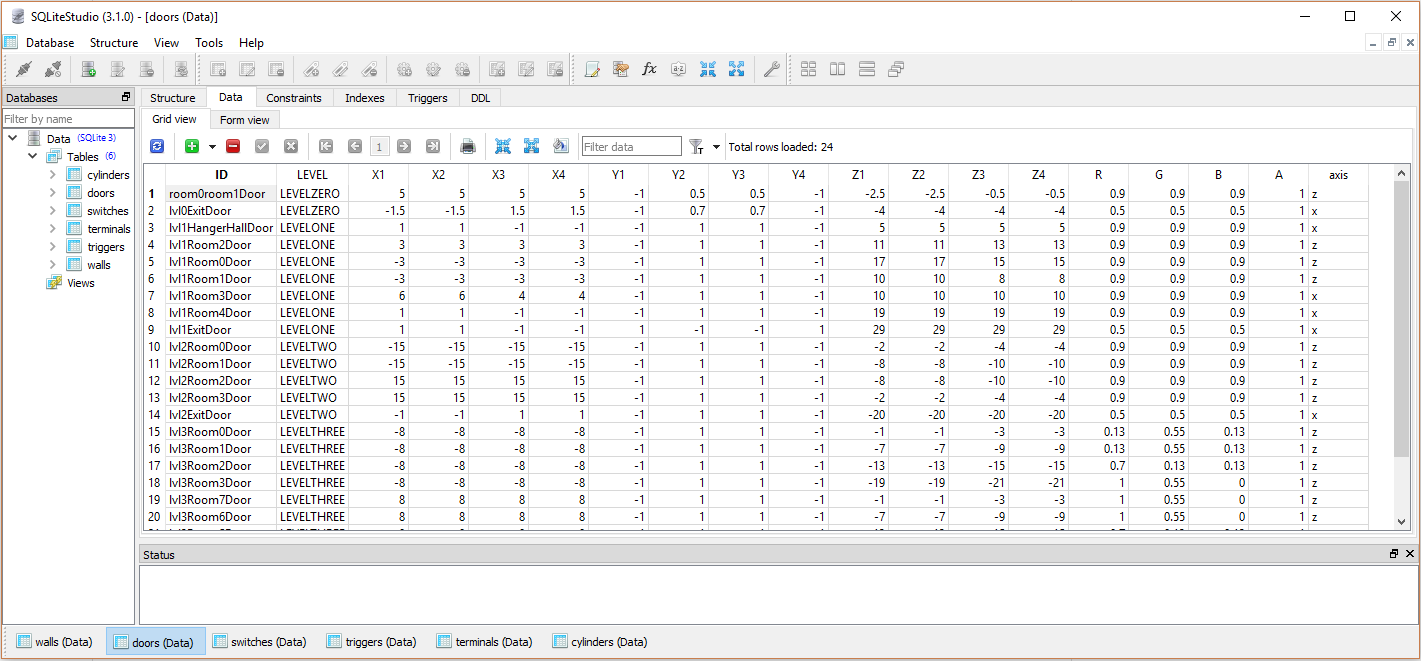
\includegraphics[width=300px]{sqlstudio}
	\caption{A picture of the \emph{doors} table in the SQLite Studio editor.}
	\label{fig:sqlstudio}
\end{figure}

\subsubsection{GitHub} \label{subsubsec:Github}

GitHub is an online Git repository that houses many open source projects. It also provides a great source control and branching system, where multiple branches can be created from a single point in the project to experiment with new features without any fear of damaging your code if they do not work out.

\section{The Project} \label{sec:game}

The project consists of two entities: the game engine and the game itself, which was developed on the engine. The engine and game are not two fully seperated entities as discussed in section \ref{subsubsec:seperation}.

\subsection{The Game Engine} \label{subsec:engine}

I developed the engine of my game in C++ during two, years starting in my second semester sophomore year and ending the first semester of my senior year. It consists of 49 C++ files, in which there are 3,308 lines of code and 1,122 lines of comments. The code can be found in the section \ref{subsec:source}, and it as also located on GitHub at \emph{https://github.com/Jerrgree/The-God-Core-Source}.

The engine reads a SQLite database (Data.db) that is housed in the same directory as the game executable, and it recognizes six tables in the database that correspond to six different types of in game objects---Walls, Doors, Cylinders, Terminals, Switches, and Triggers. Due to limitations discussed in \ref{subsubsec:seperation}, it will only properly work with a game that has five levels.

\subsubsection{Walls and Doors} \label{subsubsec:walls}

Walls are, at their heart, an OpenGL rectangle with a wrapper for additional functionality. In the same vein, Doors are simply Walls with the ability to open and close.

Internally they consist of two arrays: a four dimensional array containing the $rgba$ values and a twelve dimensional array containing the 4 $xyz$ coordinates of the rectangle's corners. 

The rectangles contain the most complex mathematics needed for collision, as the necessary calculus to correctly determine whether or not the player has collided with a rectangle involves determining if a sphere has collided with a plane in 3 Dimensional space.

In the constructor of a rectangle, after all values are initialized, the equation of the plane (Figure \ref{fig:plane}) is immediately calculated for future reference in collision detection.

\begin{figure}[H]
	$aX + bY + cZ + d = 0$
	\caption{The equation of a plane.}
	\label{fig:plane}
\end{figure}

This equation is calculated using the any three corners of the rectangle (A, B, and C) and then creating two vectors (B-A and C-a) using their dot product as show in Figure \ref{fig:rectangles}.

\begin{figure}[H]
\noindent
$
\vec{AB} = \left| \begin{array}{c}
Bx - Ax \\
By - Ay \\
Bz - Az
\end{array} \right|
\vec{AC} = \left| \begin{array}{c}
Cx - Ax \\
Cy - Ay \\
Cz - Az
\end{array} \right| \\
a = \vec{AB}_2 * \vec{AC}_3 - \vec{AB}_3 * \vec{AC}_2 \\
b = \vec{AB}_3 * \vec{AC}_1 - \vec{AB}_1 * \vec{AC}_3 \\
c = \vec{AB}_1 * \vec{AC}_2 - \vec{AB}_2 * \vec{AC}_1 \\
d = -(aAx + bAy + cAz)
$

\caption{Given three points of a rectangle (A, B, and C), the equation of the plane can be derived with the dot product of two vectors. \cite{Plane} }
\label{fig:rectangles}
\end{figure}
The norm of the plane can then be derived using the equation $\sqrt{a^2 + b^2 + c^2}$.

\subsubsection{Terminals} \label{subsubsec:terminals}

Terminals are an in-game computer that the player can access to read parts of the stories lore, as well as unlock new doors for them to explore.

Each terminal is bound to a unique \emph{terminal file} that is heavily structured and contains its data. An example is show in Figure \ref{fig:terminal}

\begin{figure}[H]
\lstinputlisting[
basicstyle=\ttfamily \small,
numbers=left,
breaklines=true,
linerange={1-1000},
firstnumber = 1]{../Resources/Text/test.tm}
\caption{An example Terminal file}
\label{fig:terminal}
\end{figure}

The program parses the file by first separating the in game content (the bracketed number and name) that should be displayed to the user from it's tag. The tags are stored in an array, where its index is equal to the bracketed number. The help display is always stored at the 0th index.

The terminal recognizes a number of commands.

\begin{itemize}
	\item Help---Displays the help prompt.
	\item Read X---Reads the requested tag. If X is zero or greater than the highest number, an error is returned.
	\item Quit or Exit---Removes the player from the terminal and back into the world.
\end{itemize}

The terminal also stores a history of what the player types, and the up and down arrows can be used to cycle through previous commands.

\subsubsection{Switches} \label{subsubsec:switch}

A switch is a button that is attached to a wall and is visible on either side. Switches are primarily bound to doors and terminals and are used to open/close a door or power on/off a terminal. Switches are also the mechanism to change levels, each level except for the last contains a switch that, when activated, will trigger a level change. Switches serve as the primary means of progress, as the level change switch and many door switches will initially be off, and the player must navigate through the level to power on more switches and progress through the level.

Internally a switch consists of two three dimension vectors, one containing its $xyz$ center and the other containing its $xyz$ rotation. It also contains a void pointer to its target and an identifier as to what type of object the target is so that the pointer can be properly typecast.

\subsubsection{Triggers} \label{subsubsec:Triggers}

Triggers are not a tangible object in the game, rather, they serve as the description of an event. Triggers are a more sophisticated form of interaction between two different objects. The implementation was designed to be abstracted away from object types so that any arbitrary object could activate another. 

The trigger holds two void pointers, one for a triggering object and one for the target object, as well as identifiers for which object type they are. Whenever an object is interacted with, every trigger in the game is tested and if the object is the same as the trigger pointer (no referencing needed as the pointers will always be equal), the target is dereferenced according to the appropriate type and activated. For the differences between triggers and switches, see section \ref{subsubsec:trigandswitch}.

\subsubsection{Cylinders} \label{subsubsec:cylinders}

Cylinders solely exist as decoration. Internally it contains the radius of each base, the height, an $xyz$ center, the $rgba$ values, and the number of "slices" or how smooth it should appear.

\subsubsection{Camera Controller} \label{subsubsec:camera}

The camera control describes how the player looks around and moves. Internally it contains the $xyz$ rotation, which describes the direction that the player is looking, and the $xyz$ coordinates where the player is physically located. The $x$ rotation corresponds to left/right movement, the $y$ coordinate refers to up/down movement, and $z$ rotation would be similar to a barrel roll.

The player can move forwards and backwards, as well as strafe left and right, in respect to the direction that they are facing. The equation to determine movement is the formula to determine a point on the circumference of a circle as seen in Figure \ref{fig:circumference}. Only the angle of x rotation is necessary for the formula, as looking left and right are the only things that impact where one would move. Given the formula, it is equally easy to implement other directions of movement by adding and subtracting 90$\degree$ from the x angle.

\begin{figure}[H]

z := z $\pm$ moveSpeed * cos(radian($\theta$)) \\ 
x := x $\mp$ moveSpeed * sin(radian($\theta$))

\caption{This equation finds an arbitrary point on a circle's circumference in relation to a specified angle. \cite{Deyoso} }
\label{fig:circumference}
\end{figure}
Following that formula, it's simple to implement movement to the left, right by adding or subtracting 90$\degree$, and backwards movement by adding 180$\degree$.

\begin{figure}[H]
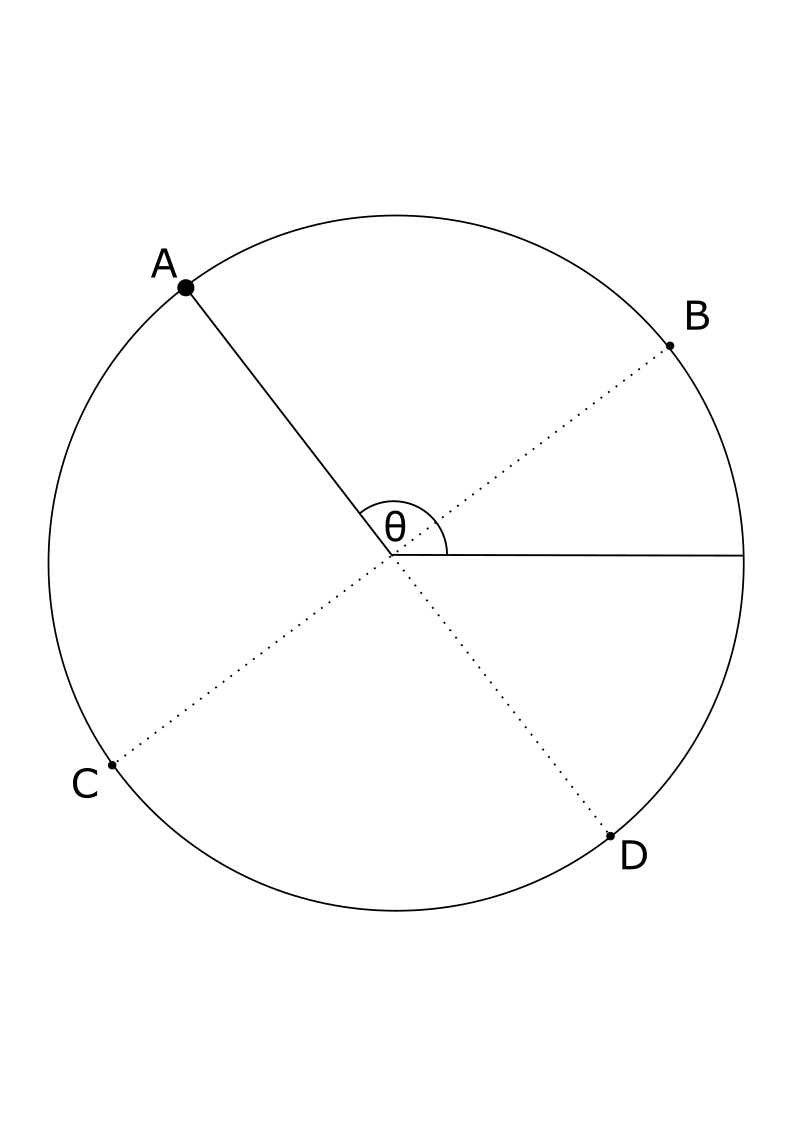
\includegraphics[width=100px]{circle}
\caption{A graphical representation of movement. With the player at the center of the circle and $\theta$ = x rotation, point A would represent forward movement, B and C would represent strafing left and right, and point D would represent backwards movement.}
\label{fig:circle}
\end{figure}

\subsubsection{Keyboard Controller} \label{subsubsec:keyboard}

The Keyboard class primarily serves to encapsulate the OpenGL callbacks that receive keystrokes: the normal function that accepts all alphanumeric and punctuation keys, and the special function that handles function keys and arrows. The keyboard function acts differently depending on what mode the player is currently in.

Under normal circumstances, the only normal keystrokes accepted are the WASD keys for movement, the E key for interaction, the '~' key for toggling the development console, and the escape key which will return the player to the main menu.

When in either a terminal or the development console, all keys are immediately concatenated to an input string with the exception of the '~' which will close the development console, or the enter key which will send the input string to it's appropriate destination to be parsed and interpreted, after which the input string is cleared so that a new command can be entered.

Also accepted are the up and down arrow keys, which will cycle through the console/terminals command history.

When the user is in the main menu, no keyboard keys are accepted other than F2, which will close the game under any circumstances.

\subsubsection{Music Controller} \label{subsubsec:musiccontroller}

To play background music, I created a class that uses the FMOD Low Level API that knows the directory that all sound files are stored and will play a designated one on infinite repeat until the prompted to change songs.

Each song in game is mapped to an integer. On each level change, the song number is incremented and a boolean flag is tripped, which signals the music controller to play the next song. Each song is dynamically allocated, so it is important to properly deallocate the songs before the next one is played. Considerations on how to change the Music Controller are noted in section \ref{subsubsec:seperation}.

\subsubsection{Text Controller} \label{subsubsec:textcontroller}

The Text Engine handles displaying all text to the screen, from prompts on the HUD to each Terminal screen. It uses OpenGL's glutBitmapCharacter function to display clear, concise text.

Every function to display text takes the $xy$ coordinates for where on the screen to start printing, and the $RGB$ color values for the text. There are two functions for displaying text, the simpler one merely takes in a string and prints it on the corresponding location on the screen. The more complex function takes in a file and a content tag which needs to be parsed. The text files are similar to terminal files as seen in Figure \ref{fig:text}.

\begin{figure}[H]
\lstinputlisting[
basicstyle=\ttfamily \small,
numbers=left,
breaklines=true,
linerange={1-1000},
firstnumber = 1]{../Resources/Text/test.txt}
\caption{An example text file, very similar to a terminal file}
\label{fig:text}
\end{figure}

The Text Engine searches through the designated file line by line until it discovers the line containing the proper tag. Then, until it reaches the closing 'END' tag, it stores every line inside of a vector. Once it has retrieved all of the necessary content, it will print the vector line by line.

\subsubsection{Collision Engine} \label{subsubsec:collision}

A \emph{collision} occurs when two or more objects in game attempt to occupy the space. The collision engine handles detecting and preventing any collision between the player and all objects in the level. In this engine there are two types of collisions: player-object collisions and player-wall collisions.

Player object collisions are simple to detect, as both the player and the object can be placed within imaginary "bounding spheres" that extend around the player and object, the collision can be detected easily using the distance formula and the radii of the spheres as seen in Figure \ref{fig:collisionsphere}.

\begin{figure}[H]
	$\sqrt{(x_2 - x_1) + (y_2 - y_1) + (z_2 - z_1)} < r_2 + r_1$
	\caption{If the distance between the sphere is shorter than the combined radii of the spheres, a collision has occurred.}
	\label{fig:collisionsphere}
\end{figure}

Player-wall collisions were much harder to reconcile. Because walls tend to be long and thin, you can't simply place one within a bounding sphere, the resulting sphere would simply be too massive and usually encompass the player entirely. 

To rectify that, the collision is split into two phases. In the first phase, we use the plane equation that is derived in the section \ref{subsubsec:walls}. Using the equation from Figure \ref{fig:wallcollision}. If the resulting value is less than the radius of the player's bounding sphere, the player is close enough to collide with that plane. However, a plane is an infinite length, and relying solely on this method would induce false collisions if the player was close to the wall but beyond it.

\begin{figure}[H]
	$\frac{ax + by + cz + d}{\sqrt{a^2 + b^2 + c^2}} < r$
	\caption{By substituting the player's $xyz$ coordinates and dividing by the norm of the plane, we can determine the distance to the plane.}
	\label{fig:wallcollision}
\end{figure}

For the second phase, each wall is aligned on an axis: x, y, or z. For the axis that it is aligned on, largest and smallest values of the coordinates are compared to the player's coordinates. palyer's corresponding coordinate is in between the two values, the player has hit the wall. Otherwise, they hit the plane but not the wall, and they do not collide.

\subsubsection{2D} \label{subsubsec:2D}

As the player's HUD, the main menu, the developer console, and terminals all need to display in a 2D environment, I extracted the ability to draw in 2D into is own class that is inherited by them in order to reduce reused code.

To convert OpenGL into 2D frame, lighting and depth masking must be disabled. Next an \emph{orthogonal} matrix is pushed onto OpenGL's matrix stack using the length and width of the screen so that all matrix transformations corresponded to a pixel on the screen. Re-enabeling 3D is as simple as popping the orthogonal matrix from the stack and re-enabling depth testing and masking.

\subsubsection{Level Management} \label{subsubsec:load}

Loading each level involves a series of operations through the SQLite API. First a connection with the database is opened, and then a series of queries are made to the database for each table in the database in turn. All important data from the database is stored in a class of the appropriate type, unnecessary data is discarded, and in the end each class is pushed into a vector of the appropriate type. 

The data is loaded in a strict order, due to some objects having dependencies on others (that is, some objects require other objects to already exist). Thus the first things that are loaded are purely independent objects, all doors, walls, cylinders, terminals. Next switches are loaded, because they require both doors and terminals to already exist. Finally, the triggers are loaded, because they require both switches and terminals.

When loading switches and triggers, the objects also need to be \emph{bound} to their appropriate required object(s). This is why doors, switches, and terminals all carry their ID's into the program with them, while triggers and walls discard their ID. Once all of the objects that need to be bound are loaded into the game, the game proceeds to bind them to their target. For each switch that needs to be bound, the game loops through the list of possible target objects and creates a pointer to the correct object inside of the switch, thus ensuring that the switch can toggle its target instantly without needing to search every time it is triggered. The triggers are bound similar, with the difference that each object must perform two searches, one for the triggering object and one for the target object.

If there is any data error in regards to binding --- that is, an object attempts to bind to an object that does not exist, the error is considered fatal and the game immediately shuts down after logging the error.

The OpenGL display function calls upon the Level class to display all in game objects. This is a simple matter, because each object knows how to display itself. Thus it is a simple matter to loop through each vector and tell each object to display itself.

\subsubsection{Game Saving and Loading} \label{subsubsec:saveload}

Game saving and loading is a simple file transaction. To save, the current level (as a string) and the song that is playing are appended to each other. The string is then encrypted and written to the save file.

Loading is a two step process. First the contents of the save file are read, decrypted, and parsed into the saved level and the saved song. Next the contents are verified so that they are valid levels to load and songs to play. If either one is invalid, the save file is considered corrupted and the game will refuse to complete the load.

\subsubsection{Console and Logging} \label{subsubsec:console}

To aid in debugging a created a Developer Console and a game log. The developer console accepts user commands to perform actions such as writing to the save file, reading the save file, disabling collision, and changing what song is playing.

The logger writes to a log file as the game runs to report on the status of operations, primarily the loading of each level. If an error occurs and the game aborts (without crashing), the appropriate error and error code is written at the end of the log file. There is only ever one log file, which is erased when the game is launched and new data is appended to it as the game runs.

\subsection{The Game} \label{subsec:thegame}

The game itself was also developed over a period of two years, starting first semester junior year and ending second semester senior year. The game itself consists of the SQLite database containging the game objects, as well as all text, terminal, image, and sound files that the game engine uses. The game is relatively short, an average play through would take 15-20 minutes, although it can easily be speed-ran in approximately five minutes.

\subsubsection{Setting} \label{subsubsec:setting}

The game takes place in the year 300x. Humanity has united under British rule, and the New British Empire has turned its eyes to colonizing the stars. The player is Special Constable Rikker, an elite agent of the Empire who has been called to scout out one of the Crown's top secret research facilities, The Daedalus, that has stopped communicating in preparation for a full investigative team that will follow behind them.

\subsubsection{Level Zero} \label{subsubsec:levelzero}

Level zero is an introductory tutorial level where the player can get a grasp with the controls. It takes place on the Constable's personal shuttle, and there is a terminal that gives access to the prior information.

\subsubsection{Level One} \label{subsubsec:levelone}

In level one, the player explores one hanger of the ship. There they can read logs detailing power outages and mechanical fluctuations, as well as security and intake reports detailing a few objects that the ship has taken on. The last report details them taking on the titular God Core.

\subsubsection{Level Two} \label{subsubsec:leveltwo}

The next level takes place in offices, where the Constable learns more about the Daedalus. It exists to house strange, unexplainable, and possibly deadly objects that are too dangerous or unknown to be left alone. Ever since taking on the God Core, crew have been slowly disappearing and communications equipment have started to fail. It comes to light that the God Core warps reality itself, and no one can determine if the missing crew has been transported elsewhere, or if they have simple disappeared from reality.

\subsubsection{Level Three} \label{subsubsec:levelthree}

Level three takes place in a gallery housing access to eight different objects. Although the Constable can only access the exhibit containing the God Core, the Constable can read information about the abilities and containment procedures for various objects.

\subsubsection{Level Four} \label{subsubsec:four}

The final level takes place in the God Core's exhibit. The player can only stare at the God Core as reality starts to deform around them, before they vanish into the unknown, ending the game.

\section{Challenges and Future Considerations} \label{sec:problemsandfuture}

\subsection{Challenges that I Faced} \subsection{challenges}

Of course, the development was not always smooth, and I did encounter plenty of problems during development.

\subsubsection{The Death of a Computer} \label{subsubsec:death}

I changed computers twice. I went from a laptop to a more powerful desktop junior year, and senior year my operating system got corrupted and I had to perform a fresh reinstall. Both times I was able to get back up to speed in only a few hours thanks to GitHub.

\subsubsection{Clipping Issues} \label{subsubsec:clipping}

OpenGL There is a problem when getting to close to a wall or a door where the player can see through parts of the wall, no doubt to do OpenGL's depth buffering in relation to distance to the wall. Part of the development processes involved balancing collision distance to the walls, at distances where the user could not see through walls the user was a noticeable distance from the wall, so I chose to allow the user to get close enough to slightly peer through the wall, as the distance felt more natural.

\subsubsection{APIs and Naming} \label{subsubsec:naming}

C++ uses unique identifiers. This means that no class, variable, or function can share the same name. Initially the Plane class was named Rectangle, as it more clearly showed that it was a wrapper for the OpenGL rectangle primitive, but when I included the Windows API I discovered that it had its own function named Rectangle, rendering my program uncompilable until I renamed every instance of my class.

\subsection{Future Considerations} \label{subsec:future}

Of course, time itself was a constraining factor, I only had two years to develop the project. As such every design choice that I made bore this limit in mind, and there portions of the engine that I was unable to optimize or implement due to lack of development time. Rarely is a project ever done, and there are always changes and improvements that could be made.

\subsubsection{Triggers and Switches} \label{subsubsec:trigandswitch}

Given time, I would have liked to implement the back end of a switch's interaction into triggers.The primary difference between triggers and switches is that a trigger is a one time activation, whereas a switch is a potentially many time toggle, but it would be a simple matter to add in different trigger types.

\subsubsection{Engine and Data Separation} \label{subsubsec:seperation}

A true game engine is fully separate from the game it runs on, however I had a few roadblocks preventing me from completely separating the two of them.

The music files and maximum song number is hard coded into the engine, as are the maximum number of levels in the game. Music and levels could easily be given their own table in the database after reworking the code that directly deals with them, but the major hurdle that led me to hard coding levels is the lack of animation. I was unable to encapsulate animation in a database, which leads to parts of the fourth level's rendering to be hard coded into the game.

\section{Acknowledgments} \label{sec:acknowledge}

I would like to offer thanks to the following people:

\begin{itemize}
	\item Kevin MacLeod, Devin Powers, and Arseniy Shkljaev for the music
	\item Robert Deyoso III for the movement equation
	\item Cody Robertson for bouncing ideas off of
	\item Brian Affolter and Lauren Ball for helping test
	\item Dr. Joshua Guerin for mentoring the project
\end{itemize}

\section{Appendices}

\subsection{Source Code} \label{subsec:source}

\subsubsection{main.cpp}
	\lstinputlisting[basicstyle=\ttfamily \small, numbers=left, breaklines=true, linerange={1-1000}, firstnumber = 1]{../main.cpp}
 				
\subsubsection{CameraControl.h}
	\lstinputlisting[basicstyle=\ttfamily \small, numbers=left, breaklines=true, linerange={1-1000}, firstnumber = 1]{../CameraControl.h}

\subsubsection{CameraControl.cpp}
	\lstinputlisting[basicstyle=\ttfamily \small, numbers=left, breaklines=true, linerange={1-1000}, firstnumber = 1]{../CameraControl.cpp}
					
\subsubsection{CollisionEngine.h}
	\lstinputlisting[basicstyle=\ttfamily \small, numbers=left, breaklines=true, linerange={1-1000}, firstnumber = 1]{../CollisionEngine.h}
					
\subsubsection{CollisionEngine.cpp}
	\lstinputlisting[basicstyle=\ttfamily \small, numbers=left, breaklines=true, linerange={1-1000}, firstnumber = 1]{../CollisionEngine.cpp}
					
\subsubsection{Console.h}
	\lstinputlisting[basicstyle=\ttfamily \small, numbers=left, breaklines=true, linerange={1-1000}, firstnumber = 1]{../Console.h}
					
\subsubsection{Console.cpp}
	\lstinputlisting[basicstyle=\ttfamily \small, numbers=left, breaklines=true, linerange={1-1000}, firstnumber = 1]{../Console.cpp}
					
\subsubsection{Cylinder.h}
	\lstinputlisting[basicstyle=\ttfamily \small, numbers=left, breaklines=true, linerange={1-1000}, firstnumber = 1]{../Cylinder.h}
					
\subsubsection{Cylinder.cpp}
	\lstinputlisting[basicstyle=\ttfamily \small, numbers=left, breaklines=true, linerange={1-1000}, firstnumber = 1]{../Cylinder.cpp}
					
\subsubsection{Door.h}
	\lstinputlisting[basicstyle=\ttfamily \small, numbers=left, breaklines=true, linerange={1-1000}, firstnumber = 1]{../Door.h}

\subsubsection{Door.cpp}
	\lstinputlisting[basicstyle=\ttfamily \small, numbers=left, breaklines=true, linerange={1-1000}, firstnumber = 1]{../Door.cpp}
 				
\subsubsection{GameManager.h}
	\lstinputlisting[basicstyle=\ttfamily \small, numbers=left, breaklines=true, linerange={1-1000}, firstnumber = 1]{../GameManager.h}

\subsubsection{GameManager.cpp}
	\lstinputlisting[basicstyle=\ttfamily \small, numbers=left, breaklines=true, linerange={1-1000}, firstnumber = 1]{../GameManager.cpp}
	 				
\subsubsection{GCTypes.h}
	\lstinputlisting[basicstyle=\ttfamily \small, numbers=left, breaklines=true, linerange={1-1000}, firstnumber = 1]{../GCTypes.h}
	 				
\subsubsection{Globals.h}
	 \lstinputlisting[basicstyle=\ttfamily \small, numbers=left, breaklines=true, linerange={1-1000}, firstnumber = 1]{../Globals.h}
	 				
\subsubsection{Globals.cpp}
	 \lstinputlisting[basicstyle=\ttfamily \small, numbers=left, breaklines=true, linerange={1-1000}, firstnumber = 1]{../Globals.cpp}
	 				
	 				
\subsubsection{HeadsUpDisplay.h}
	 \lstinputlisting[basicstyle=\ttfamily \small, numbers=left, breaklines=true, linerange={1-1000}, firstnumber = 1]{../HeadsUpDisplay.h}
	 				
\subsubsection{HeadsUpDiplay.cpp}
	 \lstinputlisting[basicstyle=\ttfamily \small, numbers=left, breaklines=true, linerange={1-1000}, firstnumber = 1]{../HeadsUpDisplay.cpp}		
	 				
\subsubsection{Keyboard.h}
	 \lstinputlisting[basicstyle=\ttfamily \small, numbers=left, breaklines=true, linerange={1-1000}, firstnumber = 1]{../Keyboard.h}
	 				
\subsubsection{Keyboard.cpp}
	 \lstinputlisting[basicstyle=\ttfamily \small, numbers=left, breaklines=true, linerange={1-1000}, firstnumber = 1]{../Keyboard.cpp}
	 				
\subsubsection{Level.h}
	 \lstinputlisting[basicstyle=\ttfamily \small, numbers=left, breaklines=true, linerange={1-1000}, firstnumber = 1]{../Level.h}
	 				
\subsubsection{Level.cpp}
	 \lstinputlisting[basicstyle=\ttfamily \small, numbers=left, breaklines=true, linerange={1-1000}, firstnumber = 1]{../Level.cpp}
	 				
\subsubsection{Logger.h}
	 \lstinputlisting[basicstyle=\ttfamily \small, numbers=left, breaklines=true, linerange={1-1000}, firstnumber = 1]{../Logger.h}
	 				
\subsubsection{Logger.cpp}
	\lstinputlisting[basicstyle=\ttfamily \small, numbers=left, breaklines=true, linerange={1-1000}, firstnumber = 1]{../Logger.cpp}
	 				
\subsubsection{MainMenu.h}
	\lstinputlisting[basicstyle=\ttfamily \small, numbers=left, breaklines=true, linerange={1-1000}, firstnumber = 1]{../MainMenu.h}

\subsubsection{MainMenu.cpp}
	\lstinputlisting[basicstyle=\ttfamily \small, numbers=left, breaklines=true, linerange={1-1000}, firstnumber = 1]{../MainMenu.cpp}	 
 				
\subsubsection{MusicManager.h}
	\lstinputlisting[basicstyle=\ttfamily \small, numbers=left, breaklines=true, linerange={1-1000}, firstnumber = 1]{../MusicManager.h}
	 				
\subsubsection{MusicManager.cpp}
	\lstinputlisting[basicstyle=\ttfamily \small, numbers=left, breaklines=true, linerange={1-1000}, firstnumber = 1]{../MusicManager.cpp}
	 				
\subsubsection{Plane.h}
	\lstinputlisting[basicstyle=\ttfamily \small, numbers=left, breaklines=true, linerange={1-1000}, firstnumber = 1]{../Plane.h}
	 				
\subsubsection{Plane.cpp}
	\lstinputlisting[basicstyle=\ttfamily \small, numbers=left, breaklines=true, linerange={1-1000}, firstnumber = 1]{../Plane.cpp}
	 			
\subsubsection{Return.h}
	\lstinputlisting[basicstyle=\ttfamily \small, numbers=left, breaklines=true, linerange={1-1000}, firstnumber = 1]{../Return.h}
	 				
\subsubsection{Resource.h}
	\lstinputlisting[basicstyle=\ttfamily \small, numbers=left, breaklines=true, linerange={1-1000}, firstnumber = 1]{../return.h}
	 				
\subsubsection{SaveManager.h}
	\lstinputlisting[basicstyle=\ttfamily \small, numbers=left, breaklines=true, linerange={1-1000}, firstnumber = 1]{../SaveManager.h}
	 				
\subsubsection{SaveManager.cpp}
	\lstinputlisting[basicstyle=\ttfamily \small, numbers=left, breaklines=true, linerange={1-1000}, firstnumber = 1]{../SaveManager.cpp}
	 				
\subsubsection{Switch.h}
	\lstinputlisting[basicstyle=\ttfamily \small, numbers=left, breaklines=true, linerange={1-1000}, firstnumber = 1]{../Switch.h}
	 				
\subsubsection{Switch.cpp}
	\lstinputlisting[basicstyle=\ttfamily \small, numbers=left, breaklines=true, linerange={1-1000}, firstnumber = 1]{../Switch.cpp}
	 				
\subsubsection{Terminal.h}
	\lstinputlisting[basicstyle=\ttfamily \small, numbers=left, breaklines=true, linerange={1-1000}, firstnumber = 1]{../Terminal.h}
	 				
\subsubsection{Terminal.cpp}	
	\lstinputlisting[basicstyle=\ttfamily \small, numbers=left, breaklines=true, linerange={1-1000}, firstnumber = 1]{../Terminal.cpp}
	 				
\subsubsection{TextEngine.h}
	\lstinputlisting[basicstyle=\ttfamily \small, numbers=left, breaklines=true, linerange={1-1000}, firstnumber = 1]{../TextEngine.h}
	 				
\subsubsection{TextEngine.cpp}
	\lstinputlisting[basicstyle=\ttfamily \small, numbers=left, breaklines=true, linerange={1-1000}, firstnumber = 1]{../TextEngine.cpp}
	 				
\subsubsection{Triangle.h}
	\lstinputlisting[basicstyle=\ttfamily \small, numbers=left, breaklines=true, linerange={1-1000}, firstnumber = 1]{../Triangle.h}
	 				
\subsubsection{Triangle.cpp}
	\lstinputlisting[basicstyle=\ttfamily \small, numbers=left, breaklines=true, linerange={1-1000}, firstnumber = 1]{../Triangle.cpp}
	 				
	 				
\subsubsection{Trigger.h}
	\lstinputlisting[basicstyle=\ttfamily \small, numbers=left, breaklines=true, linerange={1-1000}, firstnumber = 1]{../Trigger.h}
	 				
\subsubsection{Trigger.cpp}
	\lstinputlisting[basicstyle=\ttfamily \small, numbers=left, breaklines=true, linerange={1-1000}, firstnumber = 1]{../Trigger.cpp}
	 				
\subsubsection{Triple.h}
	\lstinputlisting[basicstyle=\ttfamily \small, numbers=left, breaklines=true, linerange={1-1000}, firstnumber = 1]{../Triple.h}
	 				
\subsubsection{Triple.cpp}
	\lstinputlisting[basicstyle=\ttfamily \small, numbers=left, breaklines=true, linerange={1-1000}, firstnumber = 1]{../Triple.cpp}
	 				
\subsubsection{TwoD.h}
	\lstinputlisting[basicstyle=\ttfamily \small, numbers=left, breaklines=true, linerange={1-1000}, firstnumber = 1]{../TwoD.h}

\subsubsection{TwoD.cpp}	
	\lstinputlisting[basicstyle=\ttfamily \small, numbers=left, breaklines=true, linerange={1-1000}, firstnumber = 1]{../TwoD.cpp}

\subsection{Database} \label{subsec:database}
	
\subsubsection{Walls}

\tiny{}

\setlength{\tabcolsep}{2.5pt}
\csvautolongtable[respect all]{walls.csv}

\small{}
\subsubsection{Doors}
\csvautotabular[respect all]{doors.csv}

\subsubsection{Switches}
\csvautotabular[respect all]{switches.csv}

\subsubsection{Terminals}
\csvautotabular[respect all]{terminals.csv}

\subsubsection{Triggers}
\csvautotabular[respect all]{triggers.csv}

\tiny{}
\subsubsection{Cylinders}
\csvautotabular[respect all]{cylinders.csv}

\small{}
\subsection{Images}

\subsubsection{Main Menu}
	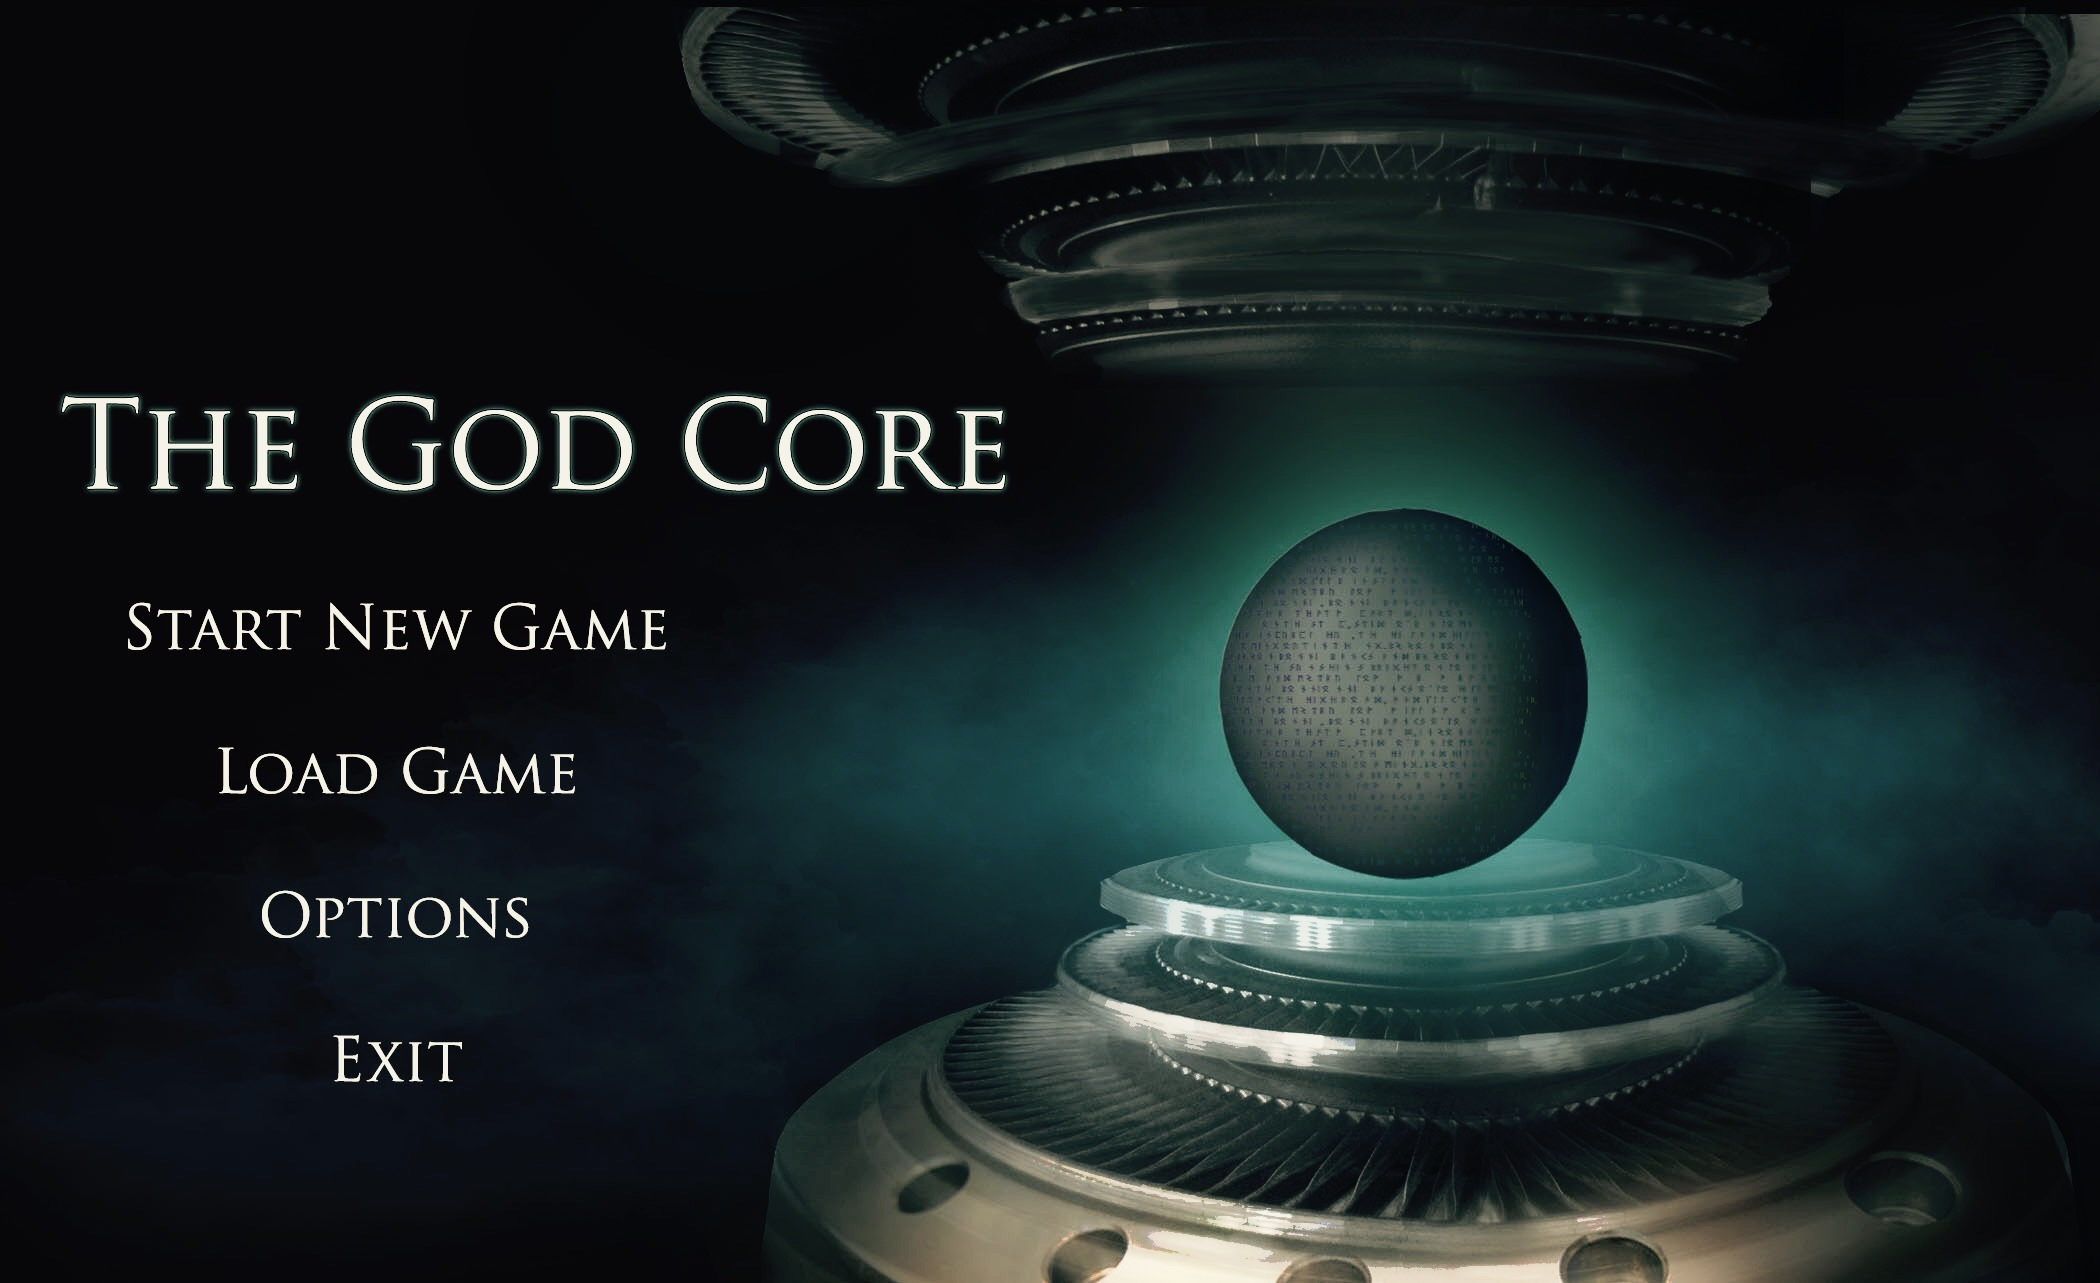
\includegraphics[width=18cm]{../Resources/Images/Main}
\subsubsection{Terminal Banner}
	
\includegraphics[width=18cm]{../Resources/Images/banner}
\subsubsection{Game Icon}
	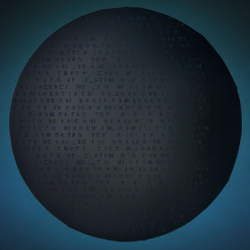
\includegraphics[width=5cm]{../Resources/Images/Core}
	
\subsection{Music}

\begin{enumerate}
	\item Dark Fog---Kevin MacLeod
	\item Mismer---Devin Powers
	\item One Sly Move---Kevin MacLeod
	\item Hypnothis---Kevin MacLeod
	\item Cold Hope---Arseniy Shkljaev
	\item Spacial Harvest---Kevin MacLeod
\end{enumerate}

\pagebreak
\begin{thebibliography}{9}

\bibitem{FMOD}
Firelight Technologies 
\textit{FMOD Studio API} \\
\textit{http://www.fmod.org/documentation/}

\bibitem{SOIL}
Jonathan Dummer
\textit{Simple OpenGL Image Library} July 7, 2008 \\
\textit{http://www.lonesock.net/soil.html}
	
\bibitem{OGL}
Khronos Group
\textit{OpenGL API Documentation Overview} \\
\textit{https://www.opengl.org/documentation/}

\bibitem{Plane}
Maplesoft
\textit{Equation of a Plane - 3 Points}

\bibitem{SHLOBJ}
Microsoft
\textit{SHGetFolderPath function} \\
\textit{https://msdn.microsoft.com/en-us/library/windows/desktop/bb762181(v=vs.85).aspx}

\bibitem{Deyoso}
Robert Deyoso
\textit{Personal Interview} February, 2015

\bibitem{sql}
SQLite Consortium
\textit{An Introduction To The SQLite C/C++ Interface} \\
\textit{https://www.sqlite.org/cintro.html}

\end{thebibliography}

\end{document}